%------------------------------------------------------------------------------
% This is a LaTeX template for the scientific justification of IRAM Proposals 
%------------------------------------------------------------------------------
% 
% We encourage IRAM proposers to use this template for the sake of unity 
% and clarity when Program Committee members assess their proposals.
% 
% You may customize this template to suit your preferences (e.g. using BibTex),
% but please respect the following requirements:
%     The scientific and technical justification should contain a 
%     maximum of 2 pages of text (4 pages for Large Programs), 
%     plus 2 pages of Figs., Tables and Refs.
%     The font size should be 11pt or larger.
%
% For Large Programs, the following sections should be included: 
%   i) Scientific Rationale, 
%  ii) Immediate Objective, 
% iii) Feasibility and Technical Justification, and 
%  iv) Organizational Issues.
%
%
%------------------------------------------------------------------------------
%
\documentclass[11pt,a4paper,twoside,graphicx,color]{article}
%
\usepackage[margin=2cm]{geometry}
\usepackage[margin=2cm]{geometry}
\usepackage[pdftex]{graphicx}
\usepackage{color}
\usepackage{txfonts}
\usepackage{paralist}
\usepackage[numbers]{natbib}
\setlength{\bibsep}{0.0pt}
\usepackage{amssymb}
\usepackage[breaklinks, colorlinks, citecolor=blue, linkcolor=MyBlue, urlcolor=RoyalPurple, colorlinks=true, linkcolor=blue, debug, baseurl=' ']{hyperref}
%
% Page size and text dimensions
% Do not change!
\textheight 260mm
\textwidth 178mm
\oddsidemargin -8mm
\evensidemargin -8mm
\marginparwidth 50pt
\topmargin -22mm
\brokenpenalty=10000
\sloppy
%
\bibpunct{(}{)}{;}{a}{}{,} 
\bibliographystyle{aa}
\definecolor{gris}{gray}{0.75}
%-------------------------------------------------------------------
\begin{document}
%
%
\begin{center}{\LARGE \bf
%-------------------------------------------------------------------
NOEMA follow-up of NIKA high-$z$ lensed galaxy candidates
%-------------------------------------------------------------------
}\end{center}
%
\centerline{\bf P.I.: R\'emi Adam \& Alexandre Beelen}

%\paragraph{Abstract (PMS only, to be removed from here)}
%High redshift dusty star forming galaxies play a fundamental role in galaxy formation and evolution. In the quest for probing these distant objects, galaxy clusters can serve as giant telescopes, thanks to the lensing magnification they produce, to observe galaxies that would be inaccessible otherwise. We propose to use NOEMA to perform the follow-up of 4 high redshift lensed dusty star forming galaxy (DSFG) candidates detected around clusters observed with NIKA+IRAM30m. These observations will allow us to check for source multiplicity, obtain high SNR and accurate position, and thus identify counterparts at other wavelengths. This project will then allow us to obtain a detailed view on the physics of DSFGs at high redshift, using a multi-wavelength approach. We will use NOEMA band 3 in configuration C for a total of 16 hours. A companion proposal was also submitted to perform a CO redshift search with EMIR+IRAM30m toward two bright lensed galaxy candidates from the same initial sample.

%\paragraph{Proposal history (PMS only, to be removed from here)}
%We have conducted Sunyaev-Zel'dovich (SZ) observations with the NIKA camera at the IRAM 30m telescope toward 6 clusters of galaxies in order to study the hot gas distribution in high redshift clusters and to prepare the NIKA2 SZ guaranteed time large program. Our primary goal, the mapping of the SZ effect at 150 GHz, was very successful and in addition our data have allowed us to detect sub-millimeter galaxies (in particular at 260 GHz), which are excellent high redshift lensed DSFG candidates. We therefore propose to follow-up a subset of these sources with NOEMA.

%%%%%%%%%%%%%%%%%%%%%%%%%%%%%%%%%%%%%%%%%%%%%%%%
\section{Scientific context}
%========== Introduction
\paragraph{\large Introduction}
Mapping the cosmic star formation history is one of the main topics of modern cosmology, on which rapid progress has been made in the last 20 years.  We now know that star formation rate (SFR) density peaked approximately 3.5 Gyr after the Big Bang \citep{Madau2014} and declined exponentially at later times, with an e-folding timescale of 3.9 Gyr. At redshift $0.5 < z < 3$, {\bf dusty star forming galaxies} (DSFGs) are dominating the history of cosmic star formation \citep[e.g.,][]{Dole2006,Burgarella2013}. At higher $z$, we are still lacking constraints on the contribution of dusty galaxy to the star formation density.  Since optical/near-infrared observations select low dust content galaxies, observations in the (sub-)millimeter range are mandatory to target these DSFGs.

Despite the growing number of detected DSFGs at high-$z$, the detailed picture of the ongoing physical processes, which control star formation in these systems (e.g., environment, merger induced starburst, accretion of cold gas, feedback processes), is still subject to many open questions \citep{Casey2014}. This is in part due to {\bf selection effects} induced by the dust obscuration of optical light that affects the corresponding surveys, or because (sub-)millimeter wide surveys mostly capture the bright end of the luminosity function of the underlying DSFG population.

%========== Lensing to probe distant galaxies
\paragraph{\large Clusters as giant telescopes to probe distant galaxies}
The quest for high-$z$ DSFGs has been extensively addressed using large (sub-)millimeter surveys such as H-ATLAS \citep{Eales2010} or SCUBA-2 CLS \citep{Geach2016}, but they generally pick-up very luminous DSFGs that are not necessarily representative of the underlying population. A way to {\bf access more typical DSFGs is to use the lensing magnification} induced by objects on the same line of sight, such as other galaxies or {\bf galaxy clusters} \citep[e.g., SPT results,][]{Vieira2013}. In large surveys, lensed DSFGs mostly arise from galaxy-galaxy lensing, but observations in the direction of clusters, aiming at capturing cluster-galaxy lensing, present several advantages: they allow for more accurate lensing modeling (necessary to correct observables from magnification); they provide an unobscured view of the background galaxies; the involved magnification factors are generally larger; and differential magnification effects are less important.

The search for bright high-$z$ lensed DSFGs has been already used at sub-millimeter wavelength using, e.g., SCUBA \citep{Knudsen2006} or the Herschel Lensing Survey \citep[HLS,][]{Egami2010}. The discovered galaxies offer a possibility of {\bf detailed multi-wavelength observations}, in which IRAM observatories have already played an important role \citep[e.g., a $z=5.2$ galaxy behind Abell 773,][]{Combes2012}.

%========== NIKA/NIKA2 SZ LP
\paragraph{\large The NIKA \& NIKA2 cluster samples and proposed observations}
The New IRAM KIDs Arrays 2 (NIKA2) has been recently installed at the IRAM 30m telescope, offering simultaneous continuum observations at 150 and 260 GHz \citep{Catalano2016}. One of the {\bf NIKA2} guaranteed time Large Programs will consist in the observation of about {\bf 50 clusters of galaxies} in the range $0.5 < z < 1$ \citep{Comis2016}. The primary goal of this program is to image the Sunyaev-Zel'dovich (SZ) signal from the clusters' hot gas at 150 GHz. However, at these redshifts, clusters also provide {\bf optimal lenses for distant background galaxies}. Therefore, we anticipate the discovery of a large number of high-$z$ lensed DSFGs at 260 GHz around the target clusters.

As a pilot project for the NIKA2 SZ large program, we have used the {\bf prototype camera, NIKA}, to successfully map six massive clusters at $0.45 < z < 0.89$ \citep{Adam2014,Adam2015,Adam2016a,Adam2016b,Ruppin2016}. We subsequently detected several DSFGs, of which many appear to be {\bf excellent high-$z$ lensed candidates}, in particular when combining NIKA and Herschel. Our brightest candidate (lensed by \mbox{CL~J1226.9+3332} at $z=0.89$, fig. \ref{fig:maps2}) was also detected in HLS and has been confirmed spectroscopically as a $z$$=$$2.4$ lensed DSFG, with EMIR \citep{Egami}.

Here, we propose to {\bf follow-up 4 lensed DSFGs candidates} selected from two of the NIKA cluster fields, {\bf using the NOEMA} band 3 (at 1.25 mm). Such observations are necessary to fully characterize the DSFGs, in particular because of the limited accuracy on the coordinates provided by NIKA. Thanks to the strong magnification of our targets, we will be able to obtain a {\bf rare view on typical DSFGs at high-$z$}. In addition, the sample will be used to optimize the scientific exploitation of NIKA2 and the observations will allow us to open up {\bf synergies between NIKA2 and NOEMA}. The cluster observations lead by our team at IRAM have been very fruitful, already resulting in 6 published/submitted papers, and this proposal is a natural continuation of this effort. A complementary companion proposal was also submitted in order to perform a CO line redshift search with EMIR at the IRAM 30m telescope, toward two of our brightest lensed DSFGs candidates from the same initial sample (tab. \ref{tab:candidate_summary}).

%%%%%%%%%%%%%%%%%%%%%%%%%%%%%%%%%%%%%%%%%%%%%%%%
\section{Technical justification}
%========== Sources selection
\paragraph{\large Sources selection and ancillary data}
Four of the six NIKA clusters are part of the CLASH sample \citep{Postman2012}, for which a {\bf wealth of multi-wavelength data} are available, including deep HST, Spitzer, Herschel/PACS+SPIRE observations, and lensing models \citep[e.g.,][]{Zitrin2015}. The two remaining ones are Planck clusters for which HST and SPIRE data are available. For all clusters, we have additional X-ray and SZ (NIKA) data, which we routinely use to infer the total cluster mass distribution, allowing us to validate magnification estimates.

To {\bf select lensed DSFG candidates}, we first built a source list by searching for compact objects in the highest magnification region around the clusters, in the {\bf NIKA maps}. We then searched for Herschel counterparts, focusing primarily on the long wavelength bands, but also considering shorter wavelengths. We extracted the NIKA and Herschel fluxes of these sources, and fit the SED with a modified blackbody spectrum \cite[see fig. \ref{fig:SED} and ][for details]{Adam2016a}. A total of 17 candidates were thus found. We note that one of them is a known lensed DSFG at $z=2.4$, measured from recent EMIR observations. Assuming that the sub-millimeter emission is dust dominated, the SED fit allows us to obtain better estimates of the flux expected in NOEMA band 3, with respect to NIKA alone. In addition, this procedure provides a first photometric redshift estimate assuming a typical dust temperature of $35 \pm 5$ K and propagating (nearly gaussian) fitting uncertainties. The source list and their properties are given in tab. \ref{tab:candidate_summary}.

Our objectives require proper $u$--$v$ coverage, to obtain unambiguous mapping inversion of the DSFGs. Therefore, we selected sources on a cluster field basis, so that they are close-by on the sky, in order to use a track-sharing observing mode among DSFGs within a cluster. The {\bf best fields} (figs. \ref{fig:maps1} and \ref{fig:maps2}), containing the best candidates in terms of redshift, magnification and SNR, are that of {\bf \mbox{CL~J1226.9+3332}} and {\bf \mbox{MACS~J0717.5+3745}} (deep NIKA data, strong magnification $\gtrsim 50$, available ancillary data). We therefore propose the observation of the brightest sources in this two fields: SMG01, SMG02, SMG07, and SMG09. We note that NOEMA data have been previously obtained toward \mbox{MACS~J0717.5+3745} at 242 GHz (1 GHz bandwidth) and two sets of $\sim 5$ hours of observations are pointed $\sim 10$" from SMG07 and SMG09 coordinates (P.I. J.P. Kneib). However, the achieved rms is expected to be a factor of 12 lower than what we aim for in this proposal at the location of our targets, and thus, do not fit our goals.

%========== Immediate objectives
\paragraph{\large Immediate objectives}
The low SNR of the millimeter detections, combined with the relatively poor angular resolution of millimeter single-dish observations prevents us to accurately measure the infrared (IR) luminosities (and SFR), the position of the sources, precisely estimate the magnification factors, and to be confident of the NIKA emission counterparts. The identification at other wavelengths of counterparts of DSFGs found with single-dish observations is very difficult. In fact, the most successful technique to circumvent this problem consists in searching for counterparts of the sources with (sub-)millimeter interferometers, as shown for example in \cite{Simpson2015}, where they locate the SCUBA-2 850 $\mu$m sources using ALMA observations at the same wavelength. In about 60\% of the ALMA maps (that are $18" \times 18"$), the single dish sources comprise the blend of $\gtrsim 2$ DSFGs. 

In this context, the proposed observations will allow us to fulfill the following immediate objectives: {\bf 1)} obtain high SNR flux measurements; {\bf 2)} check for {\bf source multiplicity}; {\bf 3)} get precise coordinates; {\bf 4)} measure precise IR luminosity and SFR. In turn, thanks to NOEMA high sensitivity and resolution, we will identify the DSFGs {\bf counterparts at other wavelengths}, construct and model the SEDs from optical to radio, and obtain precise photometric redshifts (or spectroscopic when available). It will then allow us to correct precisely for magnification and measure {\bf detailed intrinsic physical properties of these rare galaxies}. We will, in particular, study the {\bf connection between the stellar component seen in optical and the dust}, at high-$z$ \citep[see, e.g.,][]{Bouwens2016}. {\bf 5)} This project will show the potentiality of combining NOEMA+NIKA and illustrate the synergy between NOEMA and NIKA2

%========== Time and configuration
\paragraph{\large Time estimates and configuration}
Our goal is to reach a {\bf SNR $\gtrsim$ 10} on the flux of the lensed DSFGs candidates at 240 GHz, and hence, to detect them even in the case of multiplicity where the fluxes of the sub-sources are up to 30\% of the original ones \citep[in 40\% of the targets,][]{Simpson2015}. This will allow us to have SNR $\gtrsim 3$ on the faintest counterparts. Given the predicted fluxes (tab. \ref{tab:candidate_summary}) and our need for good $u$--$v$ coverage (i.e. using a {\bf track-sharing mode}), we will need 1 track per cluster field ($2 \times 8$ hours, including an overhead factor of 1.6). In the case of \mbox{CL~J1226.9+3332} sources, we should reach SNR $\sim 20$ even if the expected fluxes are $2 \sigma$ lower than the central value. This will enable a thorough validation of such pathfinder observations. 

Following \cite{Simpson2015}, the median separation between two resolved sub-sources is 1.6". We therefore choose the {\bf C configuration} to have a synthesized beam lower than 1", in order to be able to separate sub-sources in case of multiplicity. Using the PMS time estimator, we therefore request a total of {\bf 16 hours of telescope time} with band 3 (3.6 GHz bandwidth). The sources are observable $\sim 10$ hours per day during the winter semester.

%%%%%%%%%%%%%%%%%%%%%%%%%%%%%%%%%%%%%%%%%%%%%%%%
\newpage
\section{Supporting material}
%========== Table of candidates
\begin{table}[h]
\caption{\footnotesize{Summary of the properties of the lensed DSFG candidates. The 4 sources selected for the proposed observations are in bold face. The two sources proposed for EMIR observations, in order to complement this proposal, are marked by $^{\dagger}$.}}
\begin{center}
\resizebox{\columnwidth}{!} {
\begin{tabular}{c|cccc|cccccc}
\hline
\hline
Source & R.A. & Dec. & 1.15 mm flux & 2.00 mm flux & SED peak & $\beta_{\rm dust}$ & $T_{\rm eff,dust}$ & $\hat{z}_{\rm phot}$ & NOEMA B3 & $t_{\rm obs} (10 \sigma)$ \\
 & (degree) & (degree) & (mJy) & (mJy) & (GHz) & ( --- ) & (K) & ( --- ) & (mJy) & (h)\\
\hline
RXJ1347.5-1145 & \multicolumn{7}{c}{--- no strong candidate ---} \\
\hline
{\bf CLJ1226.9+3332 SMG01} & 186.74940 & 33.543114 & $8.7 \pm 1.1$ & $1.9 \pm 0.2$$^{*}$ & $816 \pm 18$ & $1.52 \pm 0.12$ & $10.3 \pm 0.5$ & $2.4 \pm 0.5$ & $7.7 \pm 0.4$ & $0.11$ \\
{\bf CLJ1226.9+3332 SMG02} & 186.75814 & 33.549083 & $3.1 \pm 1.1$ & $0.9 \pm 0.3$$^{*}$ & $609 \pm 66$ & $2.05 \pm 0.19$ & $6.7 \pm 1.0$ & $4.2 \pm 1.1$ & $3.3 \pm 0.4$ & $0.59$ \\
\hline
MACSJ1423.8+2404 SMG03 & 215.94946 & 24.070625 & $8.6 \pm 2.5$ & $-0.4 \pm 0.5$$^{**}$ & $911 \pm 88$ & $0.89 \pm 0.20$ & $14.0 \pm 1.2$ & $1.5 \pm 0.4$ & $2.3 \pm 0.4$ & $1.20$ \\
MACSJ1423.8+2404 SMG04 & 215.93582 & 24.054733 & $4.6 \pm 2.7$ & $-0.3 \pm 0.6$ & $608 \pm 792$ & $2.17 \pm 0.20$ & $6.5 \pm 10.0$ & $4.4 \pm 8.2$ & $2.0 \pm 1.1$ & $1.51$ \\
MACSJ1423.8+2404 SMG05 & 215.94742 & 24.080956 & $4.2 \pm 2.4$ & $-0.8 \pm 0.5$$^{**}$ & $751 \pm 142$ & $1.00 \pm 0.19$ & $11.1 \pm 1.8$ & $2.2 \pm 0.7$ & $2.1 \pm 0.8$ & $1.44$ \\
MACSJ1423.8+2404 SMG06 & 215.97167 & 24.062847 & $7.6 \pm 2.7$ & $0.8 \pm 0.6$ & $359 \pm 1530$ & $2.05 \pm 0.20$ & $4.0 \pm 18.9$ & $7.8 \pm 42.2$ & $4.0 \pm 0.8$ & $0.40$ \\
\hline
{\bf MACSJ0717.5+3745 SMG07} & 109.37740 & 37.745272 & $2.5 \pm 0.7$ & $0.6 \pm 0.2$$^{*}$ & $424 \pm 103$ & $1.86 \pm 0.19$ & $4.9 \pm 1.4$ & $6.1 \pm 2.3$ & $2.1 \pm 0.1$ & $1.36$ \\
MACSJ0717.5+3745 SMG08 & 109.38925 & 37.734656 & $1.5 \pm 0.7$ & $-0.1 \pm 0.2$$^{*}$ & $731 \pm 1615$ & $2.10 \pm 0.20$ & $8.0 \pm 20.0$ & $3.4 \pm 11.1$ & $0.8 \pm 0.4$ & $10.08$ \\
{\bf MACSJ0717.5+3745 SMG09} & 109.39919 & 37.759447 & $1.7 \pm 0.7$ & $0.2 \pm 0.2$$^{*}$ & $653 \pm 150$ & $2.38 \pm 0.20$ & $6.7 \pm 2.0$ & $4.2 \pm 1.7$ & $1.3 \pm 0.2$ & $3.57$ \\
MACSJ0717.5+3745 SMG10 & 109.35268 & 37.726572 & $1.4 \pm 0.9$ & $0.1 \pm 0.2$ & $865 \pm 112$ & $2.29 \pm 0.19$ & $9.0 \pm 1.5$ & $2.9 \pm 0.9$ & $0.9 \pm 0.3$ & $7.00$ \\
\hline
PSZ1G045.85+57.71 SMG11$^{\dagger}$ & 229.59864 & 29.476758 & $7.7 \pm 1.9$ & $1.6 \pm 0.4$ & $552 \pm 38$ & $1.97 \pm 0.19$ & $6.2 \pm 0.7$ & $4.6 \pm 1.0$ & $6.6 \pm 0.6$ & $0.14$ \\
PSZ1G045.85+57.71 SMG12$^{\dagger}$ & 229.59388 & 29.483133 & $8.5 \pm 2.0$ & $1.2 \pm 0.4$ & $666 \pm 37$ & $1.91 \pm 0.17$ & $7.6 \pm 0.7$ & $3.6 \pm 0.8$ & $5.9 \pm 0.7$ & $0.18$ \\
PSZ1G045.85+57.71 SMG13 & 229.57727 & 29.458097 & $4.5 \pm 1.7$ & $-0.8 \pm 0.3$$^{**}$ & $389 \pm 1570$ & $2.06 \pm 0.20$ & $4.3 \pm 19.3$ & $7.2 \pm 36.7$ & $3.9 \pm 2.3$ & $0.42$ \\
PSZ1G045.85+57.71 SMG14 & 229.59208 & 29.447528 & $3.4 \pm 1.7$ & $0.3 \pm 0.3$$^{*}$ & $801 \pm 1506$ & $0.92 \pm 0.20$ & $12.2 \pm 18.8$ & $1.9 \pm 4.5$ & $1.5 \pm 0.7$ & $2.85$ \\
\hline
PSZ1G046.13+30.75 SMG15 & 259.28271 & 24.041972 & $3.5 \pm 3.0$ & $1.2 \pm 0.5$ & $635 \pm 811$ & $1.05 \pm 0.21$ & $9.2 \pm 10.3$ & $2.8 \pm 4.2$ & $3.3 \pm 1.5$ & $0.58$ \\
PSZ1G046.13+30.75 SMG16 & 259.26292 & 24.062750 & $-1.2 \pm 2.4$ & $1.0 \pm 0.4$$^{*}$ & $762 \pm 333$ & $1.07 \pm 0.20$ & $11.0 \pm 4.3$ & $2.2 \pm 1.3$ & $2.6 \pm 0.9$ & $0.95$ \\
PSZ1G046.13+30.75 SMG17 & 259.28542 & 24.074583 & $0.0 \pm 2.3$ & $1.1 \pm 0.4$$^{*}$ & $716 \pm 860$ & $0.92 \pm 0.21$ & $10.9 \pm 10.7$ & $2.2 \pm 3.2$ & $2.4 \pm 1.2$ & $1.06$ \\
\hline
\end{tabular}
}
\end{center}
{\small {\bf Notes.} $^{*}$ Possibly contaminated by SZ signal. $^{**}$ Very likely to be contaminated by SZ signal.}
\label{tab:candidate_summary}
\end{table}

%========== Multi-lambda figure
\begin{figure}[h!]
	\centering
	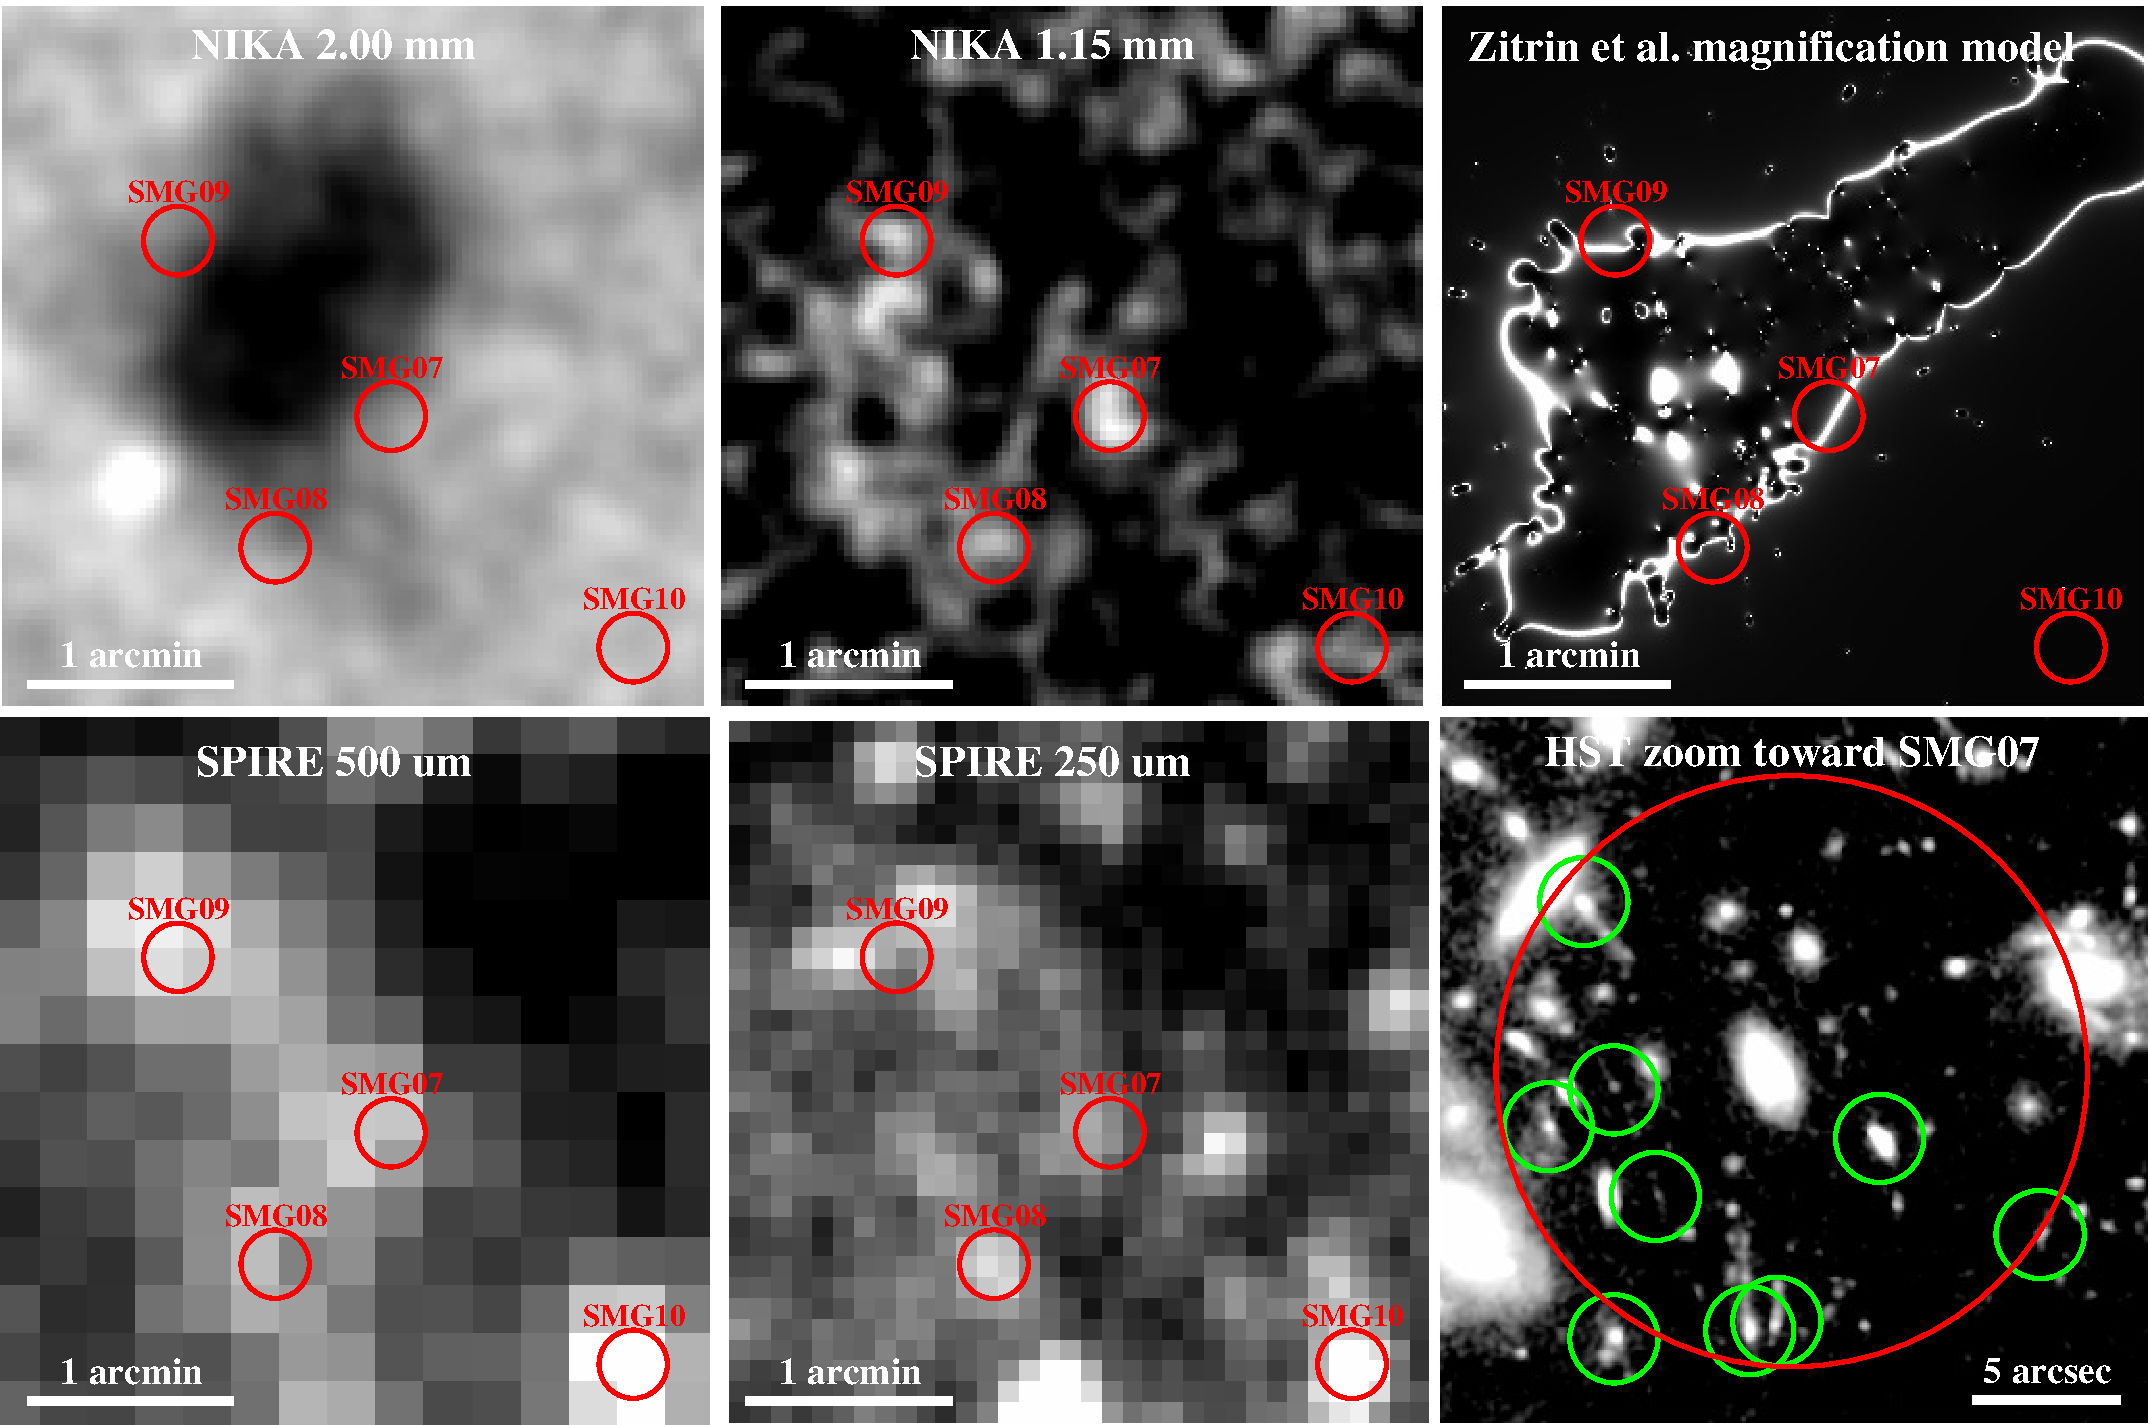
\includegraphics[width=0.69\textwidth]{MACSJ0717_multi.pdf}
	\caption{\footnotesize{{\bf Top left and top middle:} NIKA 2.00 mm (left) and 1.15 mm (right) surface brightness maps toward \mbox{MACS~J0717.5+3745}. The large scale diffuse signal is due to the SZ effect, being mostly negative at 2.00 mm and positive at 1.15 mm \citep{Adam2016b}. {\bf Bottom left and bottom middle:} SPIRE 500 and 250 $\mu$m images. {\bf Top right:} strong lensing magnification model from \cite{Zitrin2015}. {\bf Bottom right:} HST combined image zoomed in toward SMG07. All cutout are $3.4' \times 3.4'$ wide except for the bottom right field that is $24" \times 24"$ wide. The red circles are 10" radius and indicate the positions of DSFG candidates. We note that three of them happen to lie where the magnification is expected to be strong. The green circles are $1.5"$ radius and show high redshift galaxies belonging to the lensing dataset of \cite{Diego2015}, which could be matched to SMG07.}}
	\label{fig:maps1} 
\end{figure}

\begin{figure}[h!]
	\centering
	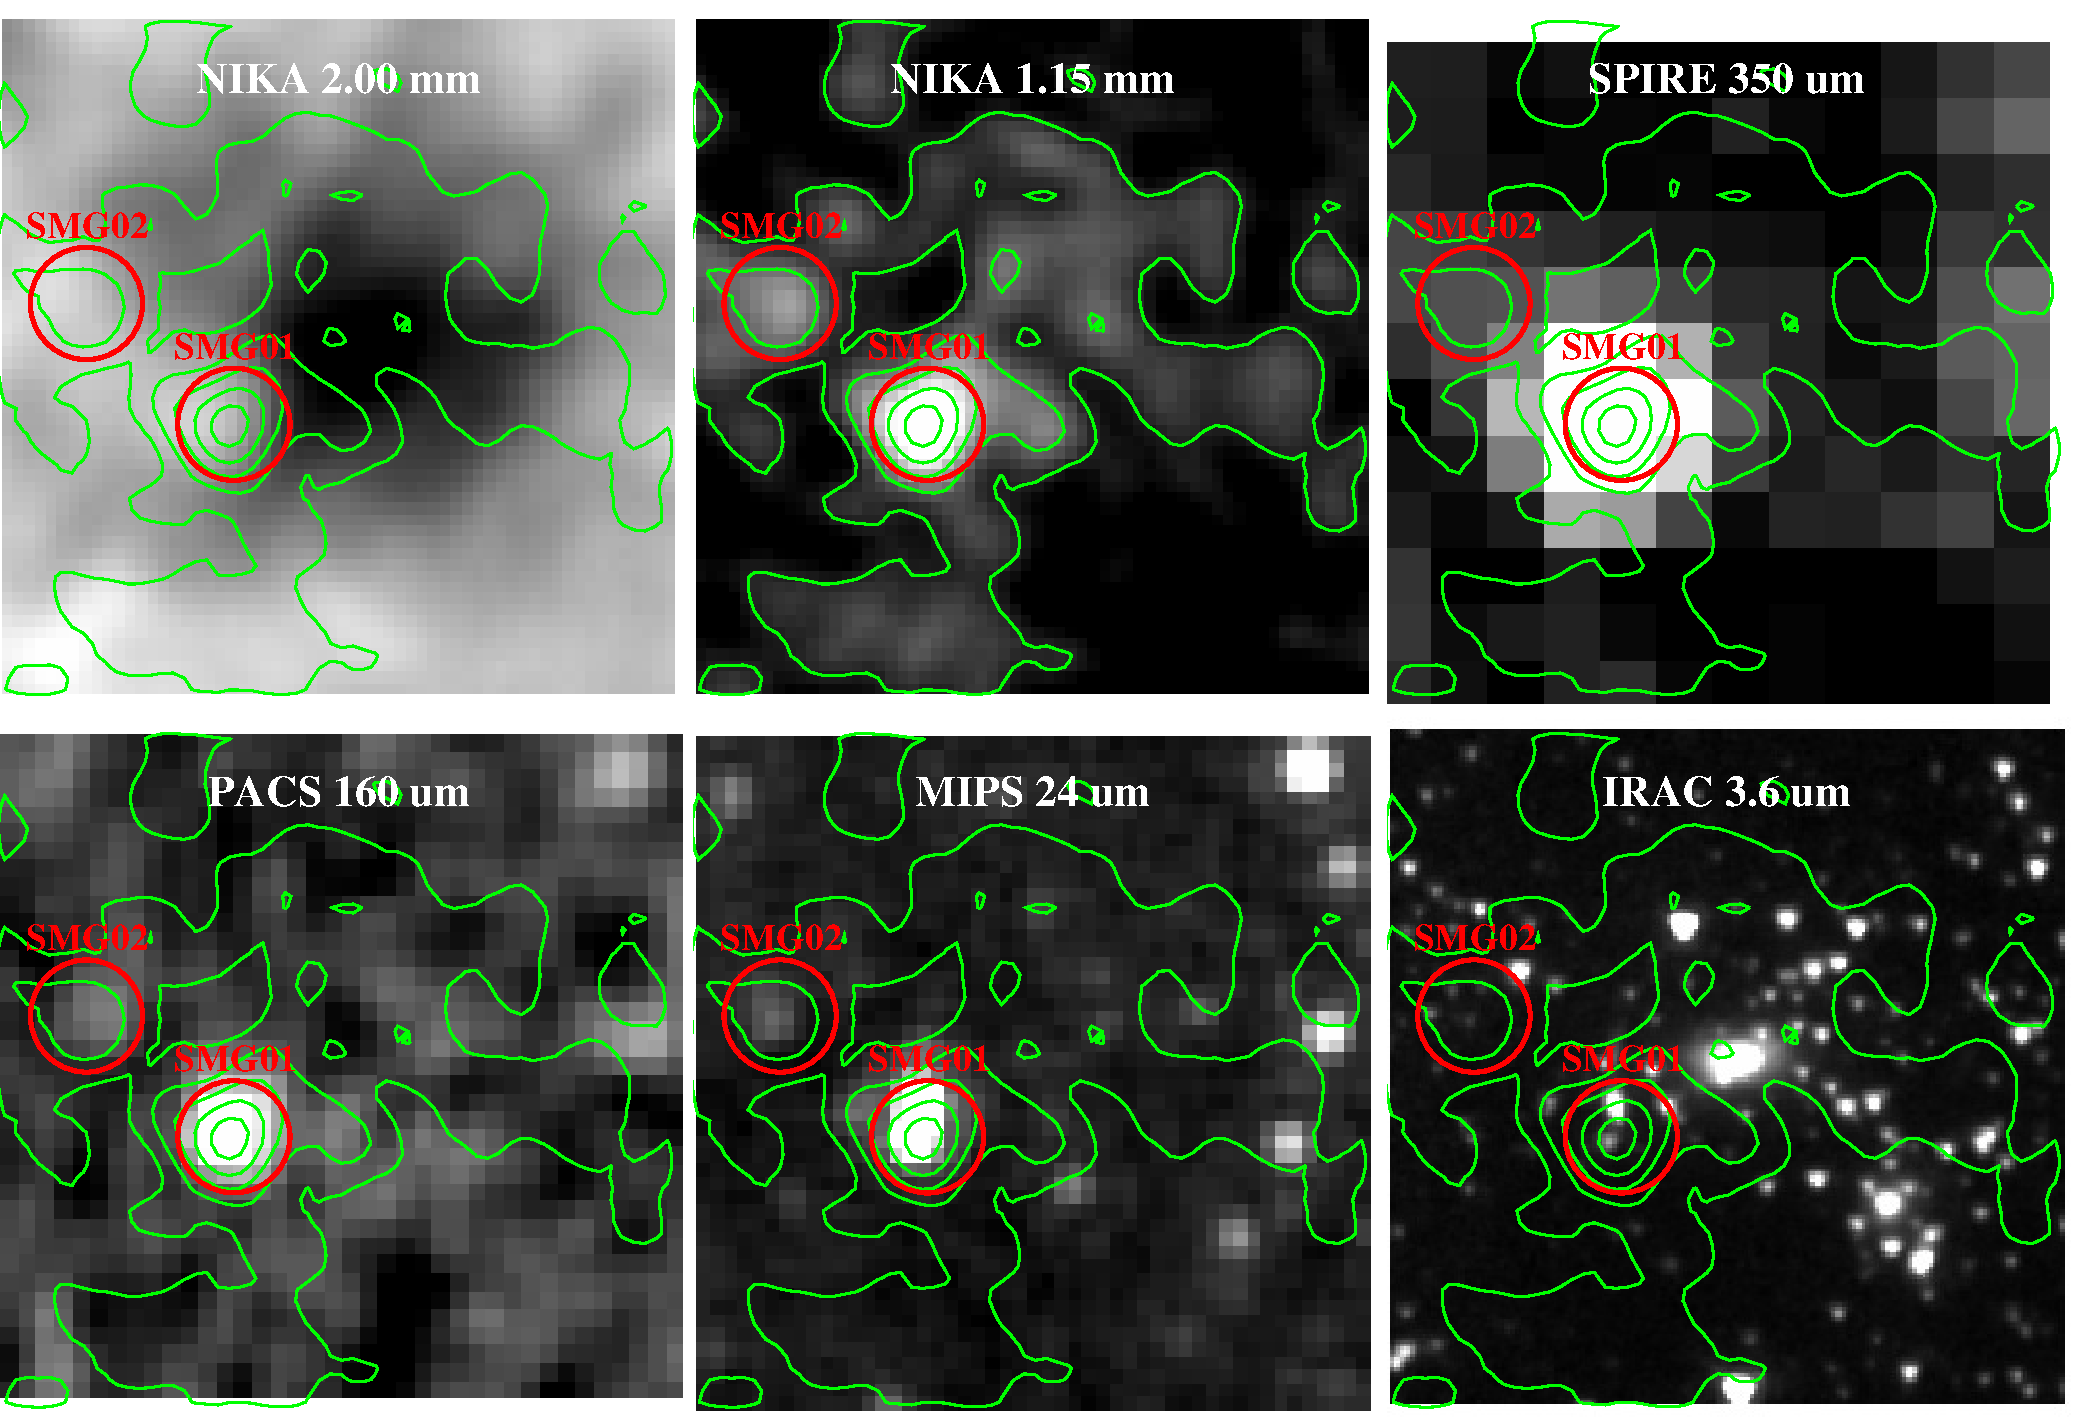
\includegraphics[trim=0cm 0cm 0cm 0.5cm, clip=true, height=6.6cm]{CLJ1227_multiL.pdf}
	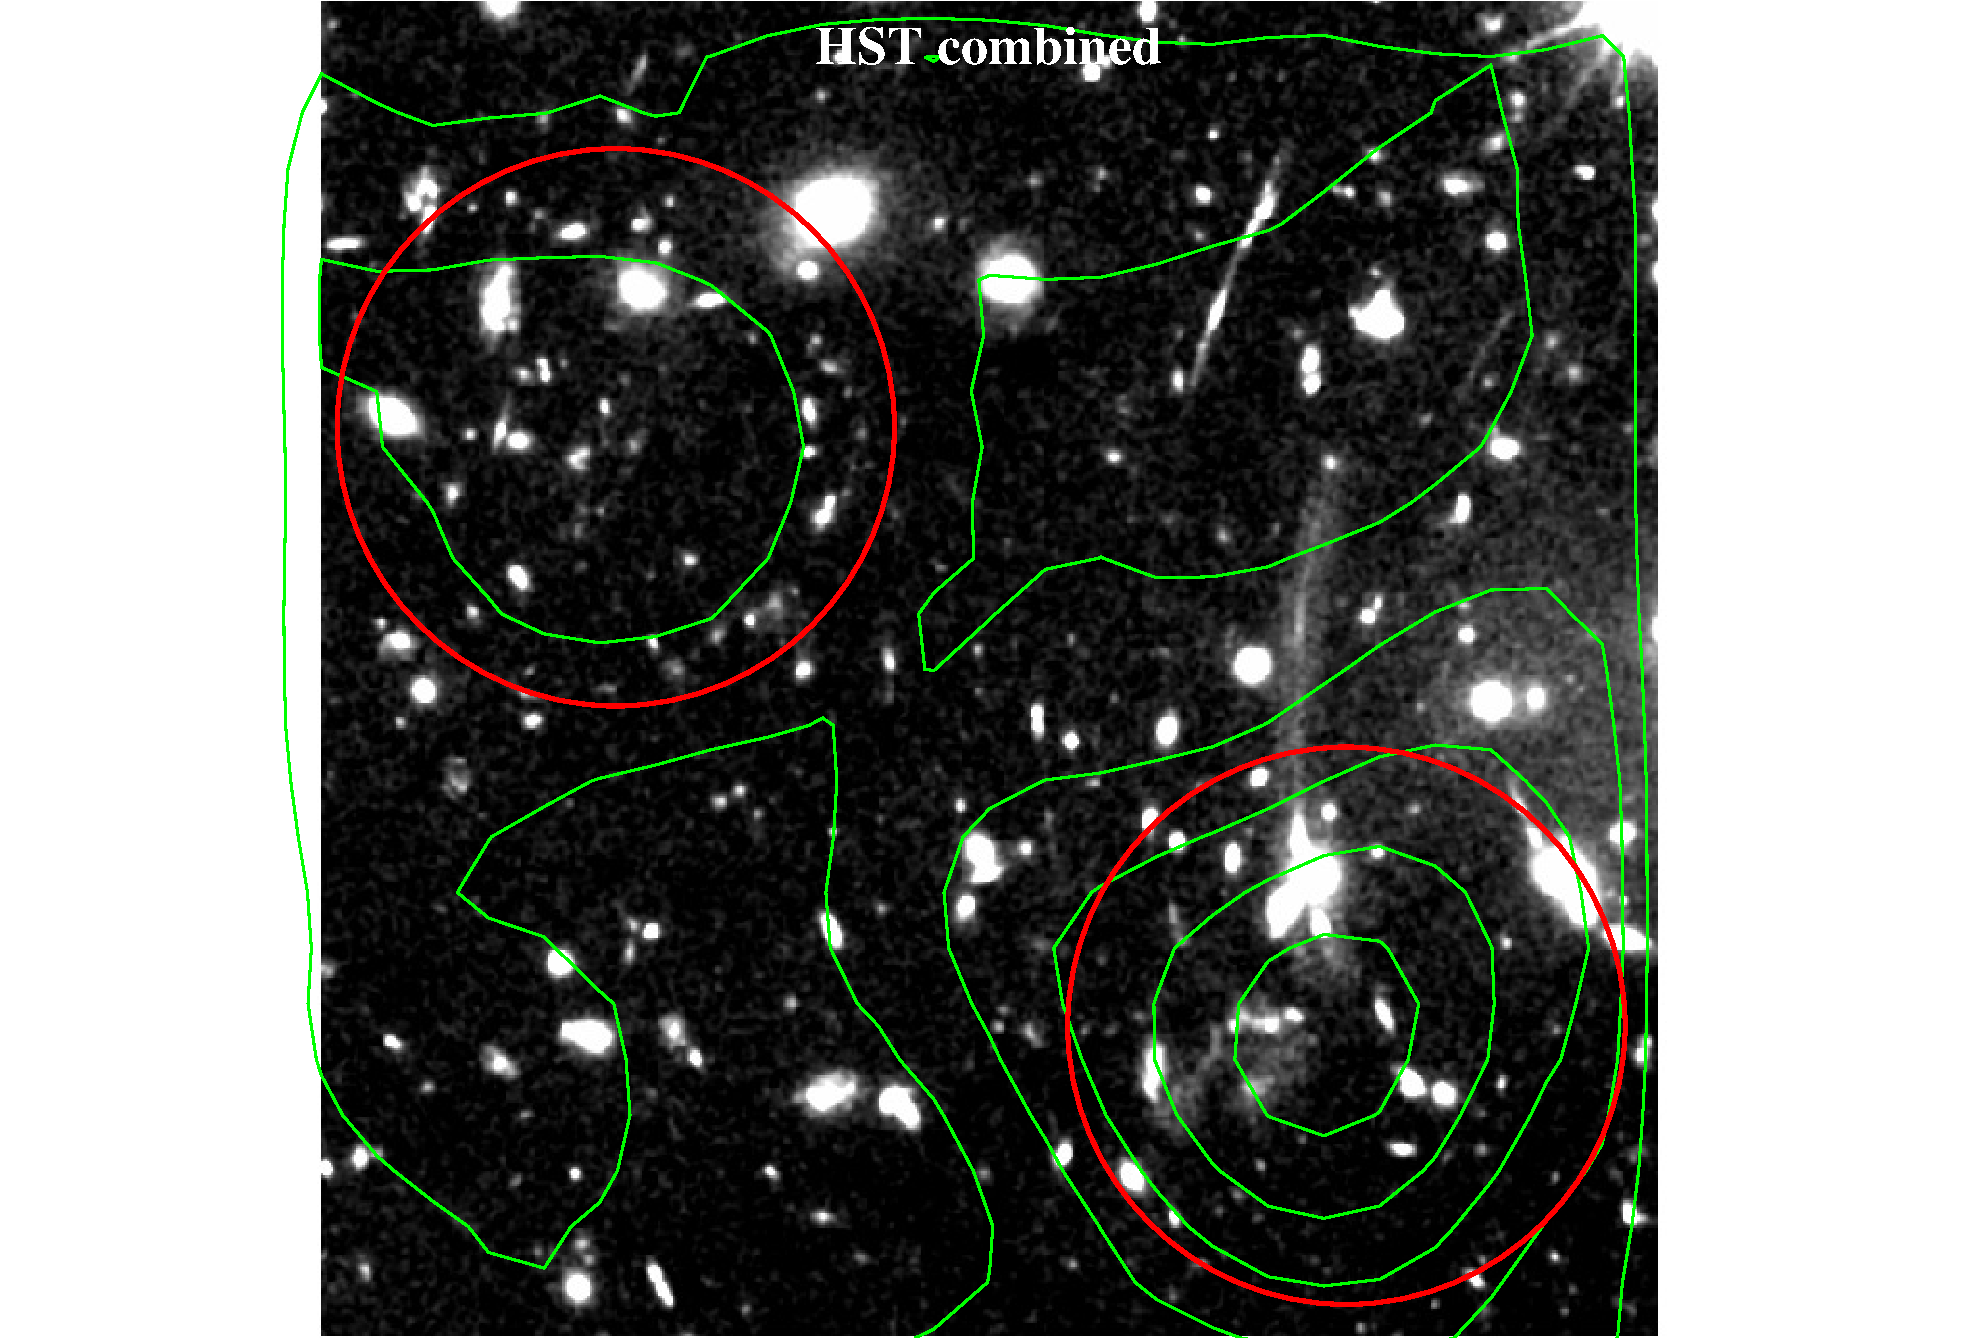
\includegraphics[trim=4.9cm 0cm 4.9cm 0cm, clip=true, height=6.6cm]{CLJ1227_HST.pdf}
	\caption{\footnotesize{Example of multi-wavelength images from millimeter to optical in the field of \mbox{CL~J1226.9+3332}. The origin/wavelength of the data are given at the top of each map. The red circles identify the two DSFG candidates in this field, SMG01 and SMG02, and the green contours provide the NIKA 1.15 mm surface brightness on a linear scale. The field of views are $2' \times 2'$ except for HST (right), which is zoomed ($0.8' \times 0.8'$) toward the DSFG candidates to highlight the presence of a giant lensing arc possibly associated with SMG01. The negative diffuse emission at 2.00 mm is due to the SZ signal, which is also visible as a positive diffuse signal at 1.15 mm, but noisier. The two DSFGs are visible from 2.00 mm to 24 $\mu$m, except maybe at 350 $\mu$m because of SPIRE limited angular resolution and confusion between SMG1 and SMG2. At higher frequencies, the high galaxy density does not allow us to reliably identify the DSFGs.}}
	\label{fig:maps2} 
\end{figure}

%========== SED figure
\begin{figure}[h!]
	\centering
	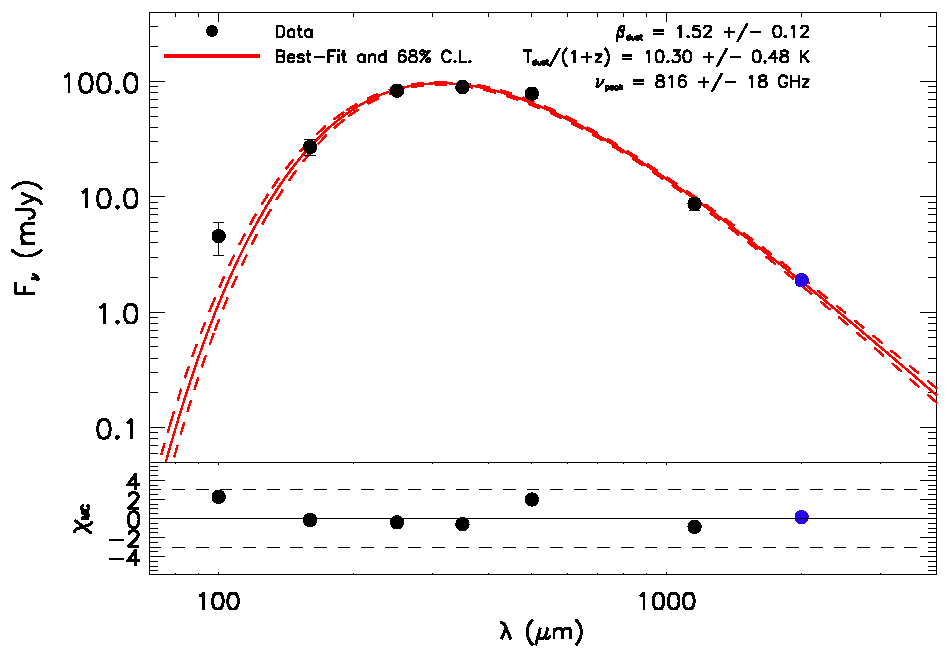
\includegraphics[width=0.49\textwidth]{SED_fit01.pdf}
	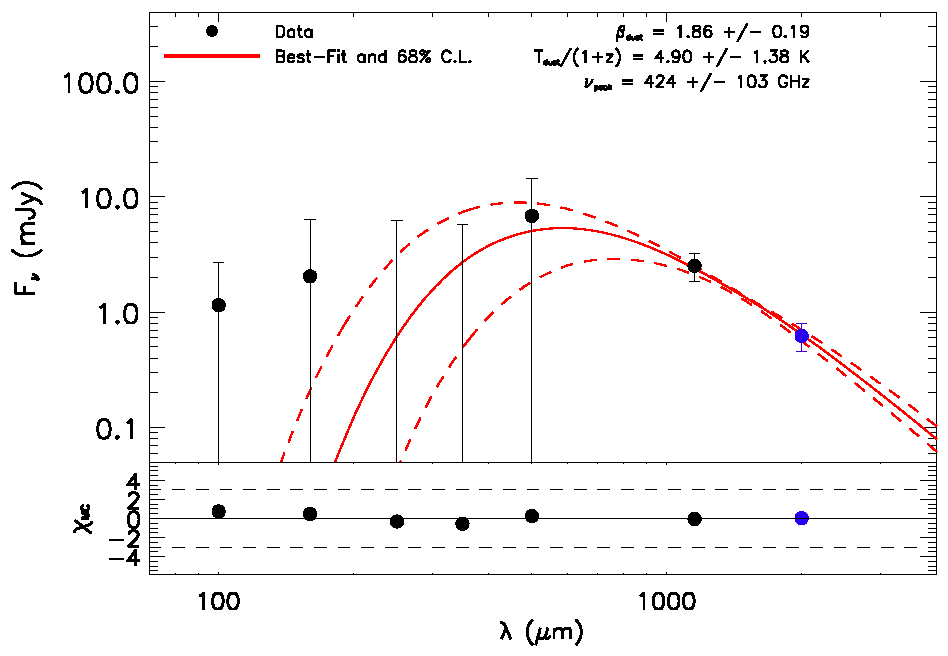
\includegraphics[width=0.49\textwidth]{SED_fit07.pdf}
	\caption{\footnotesize{Example of two NIKA+Herschel SED and their modified black-body fit constraint. The blue points indicate possible contamination from SZ signal. {\bf Left:} SMG01 (lensed by \mbox{CL~J1226.9+3332}) -- bright lensed DSFGs with confirmed redshift at $z = 2.4$ from EMIR observations. Our redshift estimates gives $\hat{z} = 2.4 \pm 0.5$ for this source. See also fig. \ref{fig:maps2}. {\bf Right:} SMG07 (lensed by \mbox{MACS~J0717.5+3745}) -- very high redshift candidate, weak in Herschel bands, but with a $>3 \sigma$ NIKA detection in the two bands despite the strong SZ signal at 2.00 mm. This source spatially coincides with several optical galaxies with $1.6 < z < 4.4$ \citep[see also][for more details]{Adam2016b}. Our redshift estimates gives $\hat{z} = 6.1 \pm 2.3$ for this source. See also fig. \ref{fig:maps1}.}}
	\label{fig:SED}
\end{figure}

%%%%%%%%%%%%%%%%%%%%%%%%%%%%%%%%%%%%%%%%%%%%%%%%
\begin{thebibliography}{9}
{\scriptsize

\bibitem[Adam et al.(2014)]{Adam2014}
R. Adam, B. Comis, J.~F. Mac\'ias-P\'erez, et al. (2014), A\&A, 569, A66, ArXiv:1310.6237

\bibitem[Adam et al.(2015)]{Adam2015}
R. Adam, B. Comis, J.~F. Mac\'ias-P\'erez, et al. (2015), A\&A, 576, A12, ArXiv:1410.2808

\bibitem[Adam et al.(2016a)]{Adam2016a}
R. Adam, B. Comis, I. Bartalucci, et al. (2016), A\&A, 586, A122, ArXiv:1510.06674

\bibitem[Adam et al.(2016b)]{Adam2016b}
R. Adam, I. Bartalucci, G.~W. Pratt, et al. (2016), A\&A, submitted, ArXiv:1606.07721
%\bibitem[Bourne et al.(2016)]{Bourne2016}
%N. Bourne, J. S. Dunlop, E. Merlin, et al. (2016), MNRAS, submitted, ArXiv:1607.04283

\bibitem[Bouwens et al.(2016)]{Bouwens2016}
R. Bouwens, M. Aravena, R. Decarli, et al. (2016), ApJ, accepted, ArXiv:1606.05280

\bibitem[Burgarella et al.(2013)]{Burgarella2013}
D. Burgarella, V. Buat, C. Gruppioni, et al. (2013), A\&A, 554, A70, ArXiv:1304.7000
	
\bibitem[Casey et al.(2014)]{Casey2014}
C.-M. Casey, D. Narayanan, \& A. Cooray (2014), Phys. Rep., 541, 45, ArXiv:1402.1456

\bibitem[Catalano et al.(2016)]{Catalano2016}
A. Catalano, R. Adam, P. Ade, et al. (2016), ArXiv:1605.08628

\bibitem[Combes et al.(2012)]{Combes2012}
F. Combes, M. Rex, T.~D. Rawle, et al. (2012), A\&A, 538, L4, ArXiv:1201.2908

\bibitem[Comis et al.(2016)]{Comis2016}
B. Comis, R. Adam, P. Ade, et al. (2016), Moriond Proceeding, ArXiv:1605.09549

\bibitem[Diego et al.(2015)]{Diego2015}
J. M. Diego, T. Broadhurst, A. Zitrin, et al. (2015), MNRAS, 451, 3920, ArXiv:1410.7019

\bibitem[Dole et al.(2006)]{Dole2006}
H. Dole, G. Lagache, J.-L. Puget, et al. (2006), A\&A, 451, 417, ArXiv:0603208

\bibitem[Geach et al.(2016)]{Geach2016}
J. E. Geach, J. S. Dunlop, M. Halpern et al. (2016), MNRAS, submitted, ArXiv:1607.03904

\bibitem[Eales et al.(2010)]{Eales2010}
S. Eales, L. Dunne, D. Clements, et al. (2010), PASP, 122, 499, ArXiv:0910.4279

\bibitem[Egami et al.(2010)]{Egami2010}
E. Egami, M. Rex, T.~D.. Rawle, et al. (2010), A\&A, 518, L12, ArXiv:1005.3820

\bibitem[Egami(priv. com.)]{Egami}
E. Egami, private communication

\bibitem[Knudsen et al.(2006)]{Knudsen2006}
K. K. Knudsen, V. E. Barnard, P. P. van der Werf, et al. 2006, MNRAS, 368, 487, ArXiv:0602131

\bibitem[Madau \& Dickinson (2014)]{Madau2014}
P. Madau \& M. Dickinson 2014, A\&ARA, 52, 415, ArXiv:1403.0007

\bibitem[Postman et al.(2012)]{Postman2012}
M. Postman, D. Coe, N. Ben\'itez, et al. 2012, ApJS, 199, 25, ArXiv:1106.3328

\bibitem[Ruppin et al.(2016)]{Ruppin2016}
F. Ruppin, R. Adam, B. Comis, et al. 2016, A\&A, submitted, ArXiv:1607.07679

\bibitem[Simpson et al.(2015)]{Simpson2015}
J.~M. Simpson, I. Smail, A.~M. Swinbank, et al. 2015, ApJ, 807, 128, ArXiv:1505.05152

\bibitem[Vieira et al.(2013)]{Vieira2013}
J.~D. Vieira, D.~P. Marrone, S.~C. Chapman, et al. 2013, Nature, 495, 344, ArXiv:1303.2723

\bibitem[Zitrin et al.(2015)]{Zitrin2015}
A. Zitrin, A. Fabris, J. Merten, et al. 2015, ApJ, 801, 44, ArXiv:1411.1414

}
\end{thebibliography}

\end{document}
